\documentclass{beamer}
\usepackage[T1]{fontenc}
\usepackage[utf8]{inputenc}

\usepackage{amsmath,amssymb,amsfonts,amsthm}
\usepackage{ulem}
% \usepackage{enumitem}

\usepackage{subcaption} % to use subfigure
\usepackage{graphicx} % to use includegraphics
\usepackage{float} % to use H
\graphicspath{{./immagini/}}    

\usepackage{tikz} % for tikzpicture
\usetikzlibrary{shapes} % node shapes
\usepackage{pgfplots} % for plots inside tikz

% setup algorithms
\usepackage[Algoritmo]{algorithm}
\usepackage[noend]{algpseudocode} % algoritmi decenti, senza end

\usetheme{Madrid}

\DeclareMathOperator{\fscore}{\mathnormal{F}-\mathnormal{Score}}

\title{Counting triangles in Data Streams}
\author[BJN]{The best team}
\institute[UniPD]{Universit\`a degli studi di Padova}
\date{2019-20}

\AtBeginSection[]
{
  \begin{frame}
    \frametitle{Table of Contents}
    \tableofcontents[currentsection]
  \end{frame}
}

\begin{document}

% define layers for pgf magic
\pgfdeclarelayer{background}
\pgfsetlayers{background,main}

\frame{\titlepage}

\begin{frame}
\frametitle{Table of Contents}
\tableofcontents
\end{frame}
 
\section{Introduzione}

%%%%%%%%%%%%%%%%%%%%%%%%%%%%%%%%%%%%%%%%%%%%%%%%%%%%%%%%%%%%%%%%%%%%%%%%%%%%%%%
\begin{frame}
\frametitle{Introduzione}
\begin{itemize}
    \item Grafi per modellare relazioni tra dati
        \begin{itemize}
            \item Reti sociali
            \item Rete internet
            \item Link tra articoli/pagine web
            \item Autori di pubblicazioni scientifiche
        \end{itemize}
\end{itemize}

\begin{itemize}
    \item Analizzare la struttura
        \begin{itemize}
            \item Analisi delle comunità
            % \item Sottografo più frequente
                % challenging computational task. The current state of the art provides methods that are either computational in- feasible on large data sets or do not provide any guarantee on the accuracy of the estimation.
            % \item Clustering coefficient
                % normalized sum of the fraction of neighbor pairs of a vertex of the graph that are connected
            \item Transitivity coefficient
                % ratio between three times the number of triangles and the number of length two paths in the graph
        \end{itemize}
\end{itemize}

\end{frame}


%%%%%%%%%%%%%%%%%%%%%%%%%%%%%%%%%%%%%%%%%%%%%%%%%%%%%%%%%%%%%%%%%%%%%%%%%%%%%%%
\begin{frame}
\frametitle{Notazione}

\begin{columns}
\begin{column}{0.5\textwidth}
    $T_0 =
    \left\{
        \left( A, B, E \right),
        \left( A, B, D \right), \dots
    \right\}$

    $T_1 =
    \left\{
        \left( A, B, C \right),
        \left( A, C, E \right), \dots
    \right\}$

    $T_2 =
    \left\{
        \left( B, C, D \right),
        \left( B, C, E \right), \dots
    \right\}$

    $T_3 =
    \left\{
        \left( C, D, E \right)
    \right\}$
\end{column}
\begin{column}{0.5\textwidth}
    \begin{center}
        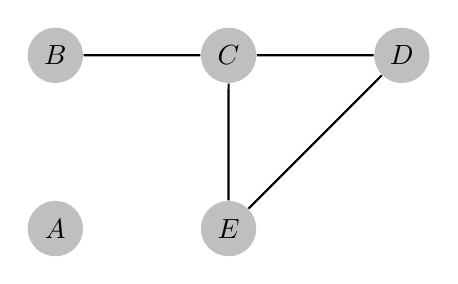
\begin{tikzpicture} [
                auto,
                swap,
                scale=1.1,
                vertex/.style={circle,fill=black!25,minimum size=20pt,inner sep=0pt},
                selected vertex/.style = {vertex, fill=red!24},
                edge/.style = {draw,thick,-},
                weight/.style = {font=\small},
                selected edge/.style = {draw,line width=5pt,-,red!50},
                outbound edge/.style = {draw,line width=5pt,-,blue!50},
                ignored edge/.style = {draw,line width=5pt,-,black!20}
            ]
        % First we draw the vertices
            \foreach \pos/\name in {
                {(0,0)/A},
                {(0,2)/B},
                {(2,2)/C},
                {(4,2)/D},
            {(2,0)/E}}
            \node[vertex] (\name) at \pos {$\name$};
        % Connect vertices with edges and draw weights
            \foreach \source/ \dest in {
            B/C, C/E, C/D, D/E}
            \path[edge] (\source) -- (\dest);
        % color a node
        % \foreach \vertex in {B, D, E}
            % \path node[selected vertex] at (\vertex) {$\vertex$};
            % \begin{pgfonlayer}{background}
            % \foreach \source / \dest in {B/C}
                % \path[outbound edge] (\source.center) -- (\dest.center);
            % \foreach \source / \dest in {D/G}
                % \path[selected edge] (\source.center) -- (\dest.center);
            % \foreach \source / \dest in {F/D}
                % \path[ignored edge] (\source.center) -- (\dest.center);
            % \end{pgfonlayer}
        \end{tikzpicture}
    \end{center}
\end{column}
\end{columns}

\end{frame}

\section{Stream non ordinato}

%%%%%%%%%%%%%%%%%%%%%%%%%%%%%%%%%%%%%%%%%%%%%%%%%%%%%%%%%%%%%%%%%%%%%%%%%%%%%%%
\begin{frame}
\frametitle{Stream non ordinato}
Struttura del grafo
\begin{itemize}
    \item non orientato
    \item gli archi appaiono nello stream in modo non ordinato
    \item ogni arco appare una sola volta nello stream
    \item non c’è il limite al grado dei nodi
    \item l’insieme $V$ e la sua taglia sono noti a priori
    \item grafo privo di self-loop (archi del tipo $e=(a,a)$)
\end{itemize}

\end{frame}

\subsection{Algoritmo a tre passate}

%%%%%%%%%%%%%%%%%%%%%%%%%%%%%%%%%%%%%%%%%%%%%%%%%%%%%%%%%%%%%%%%%%%%%%%%%%%%%%%
\begin{frame}
\frametitle{Algoritmo a tre passate}

$\Call{SampleTriangle}{ }$
\begin{enumerate}
    \item conta il numero di archi $|E|$ nello stream
    \item estrae il sample
        \begin{itemize}
            \item campionare un arco $e=(a,b)$ scelto in maniera uniforme su $E$
            \item scegliere un nodo $v$ in maniera uniforme da $V \setminus \{a,b\}$
        \end{itemize}
    \item 
        verifica la presenza degli archi mancanti
        \begin{algorithmic}
            \If {$ \left( a, v \right) \in E \vee \left( b, v \right) \in E$}
                \State $\beta \gets 1$
            \Else
                \State $\beta \gets 0$
            \EndIf
            \Return $\beta$
        \end{algorithmic}
\end{enumerate}

\end{frame}

%%%%%%%%%%%%%%%%%%%%%%%%%%%%%%%%%%%%%%%%%%%%%%%%%%%%%%%%%%%%%%%%%%%%%%%%%%%%%%%
\begin{frame}
\frametitle{Algoritmo a tre passate - analisi 1/3}

$\Call{SampleTriangle}{ }$ ritorna $\beta$ con valore atteso

\[
    \mathbb{E}[\beta]=\frac{3\left|T_{3}\right|}{\left|T_{1}\right|+2 \cdot\left|T_{2}\right|+3 \cdot\left|T_{3}\right|}
\]

\[
    \left|T_{1}\right|+2\left|T_{2}\right|+3\left|T_{3}\right|=|E| \cdot(|V|-2)
\]

\[
    % \left|T_{3}\right|
    \widetilde T_{3}
    =\mathbb{E}
    [\beta] \cdot|E| \cdot \frac{(|V|-2)}{3}
\]

\end{frame}

%%%%%%%%%%%%%%%%%%%%%%%%%%%%%%%%%%%%%%%%%%%%%%%%%%%%%%%%%%%%%%%%%%%%%%%%%%%%%%%
\begin{frame}
\frametitle{Algoritmo a tre passate - analisi 2/3}

\begin{lemma}
La stima risulta compresa tra
$
\left( 1 - \varepsilon \right)
| T_{3} |
<
\widetilde T_{3}
<
\left( 1 + \varepsilon \right)
| T_{3} |
$
con probabilità $1 - \delta$
\end{lemma}


\begin{proof}
    Utilizzando i bound di Chernoff
    \[
        \textbf{Pr}
        \left[ 
            \frac{1}{s}\sum_{i=1}^{s}\beta_i\geq(1+\epsilon)\mathbb{E}[\beta]
        \right]
        <e^{-\epsilon^2\cdot\mathbb{E}[\beta]\cdot\frac{s}{3}}
    \]
    \[
        \textbf{Pr}
        \left[ 
            \frac{1}{s}\sum_{i=1}^{s}\beta_i\leq(1-\epsilon)\mathbb{E}[\beta]
        \right]
        <e^{-\epsilon^2\cdot\mathbb{E}[\beta]\cdot\frac{s}{2}}
    \]
    si ricava
    \[
        s \geq \frac{3}{\epsilon^{2}} \cdot \frac{\left|T_{1}\right|+2\left|T_{2}\right|+3\left|T_{3}\right|}{\left|T_{3}\right|} \cdot \ln \left(\frac{2}{\delta}\right)
    \]
\end{proof}

\end{frame}


%%%%%%%%%%%%%%%%%%%%%%%%%%%%%%%%%%%%%%%%%%%%%%%%%%%%%%%%%%%%%%%%%%%%%%%%%%%%%%%
\begin{frame}
\frametitle{Algoritmo a tre passate - analisi 3/3}

Numero di istanze parallele
\[
    s \geq \frac{3}{\epsilon^{2}} \cdot \frac{\left|T_{1}\right|+2\left|T_{2}\right|+3\left|T_{3}\right|}{\left|T_{3}\right|} \cdot \ln \left(\frac{2}{\delta}\right)
\]

Utilizzo di memoria per istanza
\[
    O \left( 1 \right)
\]

Lavoro per arco dello stream (complessivo)
\[
    O\left(
    \frac{1}{\epsilon^{2}} \cdot \log \left(\frac{1}{\delta}\right) \cdot\left(1+\frac{\left|T_{1}\right|+\left|T_{2}\right|}{\left|T_{3}\right|}\right)\right)
    = O ( s )
\]

\end{frame}

%%%%%%%%%%%%%%%%%%%%%%%%%%%%%%%%%%%%%%%%%%%%%%%%%%%%%%%%%%%%%%%%%%%%%%%%%%%%%%%
\begin{frame}
\frametitle{Algoritmo a tre passate - miglioramento}

Costruendo nella seconda passata una tabella hash, si ottiene:

Utilizzo di memoria (complessivo):
\[
    O \left( s \right)
\]

Lavoro per arco dello stream (terza passata):
\[
    O ( 1 )
\]

\end{frame}

\subsection{Algoritmo a una passata}

%%%%%%%%%%%%%%%%%%%%%%%%%%%%%%%%%%%%%%%%%%%%%%%%%%%%%%%%%%%%%%%%%%%%%%%%%%%%%%%
\begin{frame}
\frametitle{Algoritmo a una passata}

\begin{itemize}
    \item Reservoir sampling
    \item $ \mathbb{E} [\beta] $ diminuisce di un fattore 3
        \[
            \mathbb{E}[\beta]=\frac{\left|T_{3}\right|}{\left|T_{1}\right|+2 \cdot\left|T_{2}\right|+3 \cdot\left|T_{3}\right|}
        \]
    \item La stima di $T_3$ risulta
        \[
            % \left|T_{3}\right|
            \widetilde T_{3}
            =\mathbb{E}
            [\beta] \cdot|E| \cdot (|V|-2)
        \]
    \item Stesso numero di istanze parallele
\end{itemize}

\end{frame}

%- - - - - - - - - - - - - - - - - - - - - - - - - - - - - -  


\section{Stream incidente}

%%%%%%%%%%%%%%%%%%%%%%%%%%%%%%%%%%%%%%%%%%%%%%%%%%%%%%%%%%%%%%%%%%%%%%%%%%%%%%%
\begin{frame}
\frametitle{Stream incidente}
Struttura del grafo
\begin{itemize}
    \item gli archi incidenti allo stesso nodo appaiono sequenzialmente nello stream
        % cioè prima arrivano gli archi incidenti al nodo 𝒗1, seguiti dagli archi incidenti al nodo 𝒗2 e così via. L’ordine di 𝒗1 , 𝒗2 , ......, 𝒗n  è arbitrario;
    \item il grafo è non orientato
    \item ogni arco appare due volte
    \item non c’è il limite al grado dei nodi e sia $d_i$ il grado del nodo $v_i$
\end{itemize}

\end{frame}

\subsection{Algoritmo a tre passate}

%%%%%%%%%%%%%%%%%%%%%%%%%%%%%%%%%%%%%%%%%%%%%%%%%%%%%%%%%%%%%%%%%%%%%%%%%%%%%%%
\begin{frame}
\frametitle{Algoritmo a tre passate}

$\Call{SampleTriangle2}{ }$
\begin{enumerate}
    \item conta il numero di triplette di nodi contenenti un cammino di lunghezza 2 nello stream
\[
    P:=\left|T_{2}\right|+3 \cdot\left|T_{3}\right|=\sum_{i=1}^{|V|} d_{i} \cdot\left(d_{i}-1\right) / 2
\]
    \item sceglie in modo uniforme una delle triplette
        usando il metodo
        $\Call{UniformTwoPath}{ }$
        e sia $(a, v, b)$ la tripletta selezionata;
    \item 
        verifica la presenza dell'arco $(a,b)$ nello stream
        \begin{algorithmic}
            \If {$ \left( a, b \right) \in E$}
                \State $\beta \gets 1$
            \Else
                \State $\beta \gets 0$
            \EndIf
            \Return $\beta$
        \end{algorithmic}
\end{enumerate}

\end{frame}

%%%%%%%%%%%%%%%%%%%%%%%%%%%%%%%%%%%%%%%%%%%%%%%%%%%%%%%%%%%%%%%%%%%%%%%%%%%%%%%
\begin{frame}
\frametitle{Metodo UniformTwoPath}

Due approcci di implementazione:
\begin{itemize}
    \item reservoir sampling
    \item avendo a disposizione $P$, si può selezionare il $k$-esimo path di lunghezza $2$ in modo randomizzato. Più alto è il grado del nodo più alta è la probabilità di essere selezionato.
\end{itemize}

\end{frame}

%%%%%%%%%%%%%%%%%%%%%%%%%%%%%%%%%%%%%%%%%%%%%%%%%%%%%%%%%%%%%%%%%%%%%%%%%%%%%%%
\begin{frame}
\frametitle{Algoritmo a tre passate - analisi}

$\Call{SampleTriangle2}{ }$ ritorna $\beta$ con valore atteso

\[
    \mathbb{E}|\beta|=\frac{3 \cdot\left|T_{3}\right|}{\left|T_{2}\right|+3 \cdot\left|T_{3}\right|}
\]

Per ottenere una $(\varepsilon, \delta)$-approssimazione, bisogna eseguire l'algoritmo almeno $s$ volte, e il valore si ricava con i bound di Chernoff
\[
    s \geq \frac{3}{\epsilon^{2}} \cdot \frac{\left|T_{2}\right|+3 \cdot\left|T_{3}\right|}{\left|T_{3}\right|} \cdot \ln \left(\frac{2}{\delta}\right)
\]

La stima risulta
\[
    \widetilde{T_{3}}:=\left(\frac{1}{s} \cdot \sum_{i=1}^{s} \beta_{i}\right) \cdot\left(\sum_{i=1}^{|V|} d_{i} \cdot\left(d_{i}-1\right)\right) / 6
\]

\end{frame}

\subsection{Algoritmo a una passata}

%%%%%%%%%%%%%%%%%%%%%%%%%%%%%%%%%%%%%%%%%%%%%%%%%%%%%%%%%%%%%%%%%%%%%%%%%%%%%%%
\begin{frame}
\frametitle{Algoritmo a una passata}

L’algoritmo a tre passate viene compresso ad una passata come segue:
\begin{itemize}
    \item Non conoscendo a priori $P$, si trova una guess $\widetilde{P}$ tale che $P \leq \widetilde{P} < 2P$.
        Il sampling potrebbe fallire con probabilità al massimo $1/2$, cioè si seleziona una tripletta non contenente il cammino di lunghezza 2; ciò introduce un fattore 2 nel calcolo di $\beta$
    \item Si combinano la seconda e la terza passata, ovvero dopo aver selezionato la tripletta $(a, v, b)$, nella stessa passata dello stream si comincia a testare se $(a, b) \in E$. Questo introduce un fattore 1/3 nella stima di $\beta$
\end{itemize}

\end{frame}


%%%%%%%%%%%%%%%%%%%%%%%%%%%%%%%%%%%%%%%%%%%%%%%%%%%%%%%%%%%%%%%%%%%%%%%%%%%%%%%
\begin{frame}
\frametitle{Algoritmo a una passata - analisi}

$\Call{SampleTriangle2\_OnePass}{ }$ ritorna $\beta$ con valore atteso

\[
    \mathbb{E}|\beta|=\frac{2 \cdot \left|T_{3}\right|}{\left|T_{2}\right|+3 \cdot\left|T_{3}\right|}
\]

Per ottenere una $(\varepsilon, \delta)$-approssimazione, bisogna eseguire l'algoritmo almeno $s$ volte, e il valore si ricava con i bound di Chernoff
\[
    s \geq \frac{3}{\epsilon^{2}} \cdot \frac{\left|T_{2}\right|+3 \cdot\left|T_{3}\right|}{\left|T_{3}\right|} \cdot \ln \left(\frac{2}{\delta}\right)
\]

La stima risulta
\[
    \widetilde{T_{3}}:=\left(\frac{1}{s} \cdot \sum_{i=1}^{s} \beta_{i}\right) \cdot\left(\sum_{i=1}^{|V|} d_{i} \cdot\left(d_{i}-1\right)\right) / 4
\]

\end{frame}

\section{Implementazione ottimizzata}

%%%%%%%%%%%%%%%%%%%%%%%%%%%%%%%%%%%%%%%%%%%%%%%%%%%%%%%%%%%%%%%%%%%%%%%%%%%%%%
\begin{frame}
\frametitle{Tecniche utilizzate}

\begin{itemize}
    \item Hash function:
utilizzate per trovare velocemente elementi in un insieme
    \item Uniform Sample Selection:
        \begin{itemize}
            \item variante del reservoir sampling
            \item estrazione di r elementi uniformemente distribuiti
        \end{itemize}
    \item Draw sample:
        non decidere per ogni elemento se verrà considerato nel sample:
        quando un elemento viene selezionato, si estrae l'indice dell'elemento successivo da selezionare
\end{itemize}
\end{frame}

%%%%%%%%%%%%%%%%%%%%%%%%%%%%%%%%%%%%%%%%%%%%%%%%%%%%%%%%%%%%%%%%%%%%%%%%%%%%%%%
\begin{frame}
\frametitle{Stream non ordinato - una passata}

Considera $r$ sample alla volta

Mantiene le strutture
\begin{itemize}
    \item $S$: tabella hash di archi mancanti
    \item $M$: stima del numero di archi nello stream
\end{itemize}

\end{frame}

%%%%%%%%%%%%%%%%%%%%%%%%%%%%%%%%%%%%%%%%%%%%%%%%%%%%%%%%%%%%%%%%%%%%%%%%%%%%%%%
\begin{frame}
\frametitle{Stream non ordinato - una passata - dettagli}

Per ogni edge dello stream
\begin{enumerate}
    \item se è quello indicato dal draw sampling:
        \begin{itemize}
            \item seleziona un nodo
            \item aggiunge i due edge mancanti nella hash table
            \item imposta a 0 un contatore per questo sample
        \end{itemize}
    \item 
verifica se deve aggiustare i sample per mantenere probabilità uniforme
    \item 
controlla se l'edge corrente è uno dei mancanti dei sample esistenti
% sfrutta l'hash table
\end{enumerate}

Per ogni sample, controlla se entrambi gli edge mancanti sono stati visti
% (contatore a 2)

\end{frame}

%%%%%%%%%%%%%%%%%%%%%%%%%%%%%%%%%%%%%%%%%%%%%%%%%%%%%%%%%%%%%%%%%%%%%%%%%%%%%%%
\begin{frame}
\frametitle{Stream ordinato - una passata}

Considera $r$ sample alla volta

Mantiene le strutture
\begin{itemize}
    \item $D$: lista di adiacenza di un nodo
    \item $S$: sample di path lunghezza 2
    \item $P$: numero di path di lunghezza 2 visti
\end{itemize}

\end{frame}

%%%%%%%%%%%%%%%%%%%%%%%%%%%%%%%%%%%%%%%%%%%%%%%%%%%%%%%%%%%%%%%%%%%%%%%%%%%%%%%
\begin{frame}
\frametitle{Stream ordinato - una passata - dettagli}

Per ogni edge relativa a un nodo:

\begin{enumerate}
    \item 
Aggiorna la lista di adiacenza del nodo
        \begin{itemize}
            \item 
Aggiorna il numero di path di lunghezza 2
        \end{itemize}
    \item 
Se è l'edge indicato dal Draw Sample:
        \begin{itemize}
            \item 
Calcola il path da aggiungere al sample
            \item 
Genera l'indice del prossimo sample
        \end{itemize}
    \item 
Se l'indice del prossimo sample è maggiore della stima usata nella Uniform Sample Selection:
        \begin{itemize}
            \item 
Aggiorna i sample per mantenere la probabilità uniforme
        \end{itemize}
\end{enumerate}

Infine, calcola il numero di triangoli visti

\end{frame}

\section{Esperimenti computazionali - risultati}

%%%%%%%%%%%%%%%%%%%%%%%%%%%%%%%%%%%%%%%%%%%%%%%%%%%%%%%%%%%%%%%%%%%%%%%%%%%%%%%
\begin{frame}
\frametitle{Esperimenti computazionali}

Tipologie esaminate: tutte molto sparse
\begin{itemize}
    \item webgraph
    \item actors, authors, network of routers
    \item struttura dei link di Wikipedia
\end{itemize}

Dimensioni
\begin{itemize}
    \item 10k - 500k nodi
    \item 100k - 50M archi
\end{itemize}

Parametri
\begin{itemize}
    \item $r$ = (1.000), 10.000, 100.000, 1.000.000
    \item tre esperimenti per tipologia
\end{itemize}

\end{frame}

%%%%%%%%%%%%%%%%%%%%%%%%%%%%%%%%%%%%%%%%%%%%%%%%%%%%%%%%%%%%%%%%%%%%%%%%%%%%%%%
\begin{frame}
\frametitle{Risultati}

Stream non ordinato

\begin{itemize}
    \item per $r = 10.000$ non ha identificato triangoli in alcuni esperimenti
\end{itemize}

Stream ordinato

\begin{itemize}
    \item identifica più triangoli
    \item buona approssimazione (5\%) anche con $r=10.000$
\end{itemize}

\end{frame}


%%%%%%%%%%%%%%%%%%%%%%%%%%%%%%%%%%%%%%%%%%%%%%%%%%%%%%%%%%%%%%%%%%%%%%%%%%%%%%%
\begin{frame}
\frametitle{Ringraziamenti}

Grazie per l'attenzione

\end{frame}

\end{document}
